%!TEX program = xelatex
%%%%%%%%%%%%%%%%%%%%%%%%%%%%%%%%%%%%%%%%%%%%%%%%%%%%%%%%%%%%%%%%%%%%%%%%%%%%%%%%%
%
% This is a very basic template for mathematical presentations using LaTeX and beamer, aimed at University of Edinburgh students on the Honours Analysis course 2017-2018, for their "Skills" presentations.
%
% This template is just to get you started and to see what the possibilities are.  There is no required format, and you are free to use, discard, edit as much as you like.  I've put in some mathematical content to demonstrate the very basics of LaTeX.  Clearly, you will need to change this.
%
% Except for a few structural comments, I don't comment on the LaTeX itself.  If you have used it before, most of what you know should apply as usual.  If you have not, have a look at the source code, the output, and experiment with editing the code and see what happens.  Most LaTeX code is pretty intuitive, e.g. the command to produce an alpha is \alpha, the command for an integral sign is \int, etc.  You can learn an awful lot by guesswork, trial and error, and google.  
%
% The percent signs "%" are comment signs, and instruct LaTeX to ignore everything following the sign on the same line.  They can be used to comment on the code.
%
%%%%%%%%%%%%%%%%%%%%%%%%%%%%%%%%%%%%%%%%%%%%%%%%%%%%%%%%%%%%%%%%%%%%%%%%%%%%%%%%
%
% The following lines are the preamble.  They help LaTeX set-up the document, but do not print anything yet.

\documentclass{ctexbeamer}		% This tells LaTeX the document will be a "beamer" presentation

\usetheme{Madrid}		% Sets basic formatting.  Lots of options, google "beamer themes"

\usepackage{tikz}
\usepackage[colorlinks,linkcolor=blue]{hyperref}
%%% logo
\pgfdeclareimage[height=0.8cm]{logo}{./logo.png}
\logo{\pgfuseimage{logo}}
%\logo{\vspace*{-0.3cm}\pgfuseimage{logo}}


\usecolortheme{dolphin}	% Sets the colour scheme.  Lots of options, google "beamer color themes"

%\setbeamertemplate{navigation symbols}{}
% Manually changes one piece of formatting.  See what the difference is by commenting this line out.

\date{}	% Insert the date of your presentation. \today gives an unsurprising automatic date.

\title[String]{KMP}	% Insert your title.  Depending on the theme you choose above, a "short title" might be useful, as it will appear on the footer of each slide.

\author[calabash\_boy]{calabash\_boy} % Insert your name

\date{\today}

\begin{document} 	% Let's begin

% Presentations come in slide frames.  You have to tell LaTeX when to start a frame, and when to end the frame.  The most common error beginners make with beamer is forgetting the \end{frame} command.	

\begin{frame}	

\titlepage	% Prints a title page populated with the information given in the preamble
	
\end{frame}		



\begin{frame}{基础定义}	

\begin{block}{字符串}	% There are lots of "theorem-like" environments for beamer just as 	usual with LaTeX: definition, theorem, lemma, example, proof, etc...

$S$:无特殊说明,字符串仅由26个小写字母'a'-'z'构成,并用大写字母表示一个字符串。

$|S|$:表示一个字符串的长度。

$S[i]$:表示字符串\textit{S}第\textit{i}个位置的字母,下标从1开始。

\end{block}

\pause

\begin{block}{子串}

$S[l,r]$:表示字符串\textit{S}从第\textit{l}到第\textit{r}个字母顺次连接而成的新字符串。

$Prefix_{S}[i]$:表示字符串\textit{S}的长度为\textit{i}的前缀,$Prefix_{S}[i] = S[1,i]$

$Suffix_{S}[i]$:表示字符串\textit{S}的长度为\textit{i}的后缀,$Suffix_{S}[i] = S[|S| - i + 1, |S|]$

\hphantom{ }

\textbf{注意},如果语境中只存在一个字符串,则可以简写为$Prefix[i]$与$Suffix[i]$

\end{block}

\end{frame}

\begin{frame}{重要定义}

\begin{block}{\textbf{Border}}

如果字符串\textit{S}的同长度的前缀和后缀完全相同,即$Prefix[i] = Suffix[i]$则称此前缀(后缀)为一个Border(根据语境,有时Border也指长度)。

\hphantom{ }

\textbf{特殊地},字符串本身也可以是它的Border,具体是不是根据语境判断。

\end{block}

\pause

\begin{block}{例子}

若S = bbabbab,试求所有Border

\end{block}

\end{frame}

\begin{frame}{重要定义}

\begin{definition}{周期和循环节}

对于字符串\textit{S}和正整数\textit{p},如果有$S[i] = S[i-p]$,对于$p < i\le |S|$成立,则称\textit{p}为字符串\textit{S}的一个周期。

\hphantom{ }

\textbf{特殊地},$p = |S|$一定是\textit{S}的周期

\end{definition}

\pause

\begin{definition}

若字符串\textit{S}的周期\textit{p}满足\textit{p} \textbf{|} $|S|$,则称\textit{p}为\textit{S}的一个循环节

\hphantom{ }

\textbf{特殊地},$p = |S|$一定是\textit{S}的循环节

\end{definition}

\end{frame}

\begin{frame}{重要性质}

\begin{block}{Border vs 周期}

\textit{p}是\textit{S}的周期 $\Leftrightarrow |S| - p$ 是 \textit{S}的Border 

\end{block}

\pause

\begin{proof}
    \textit{p}为\textit{S}的周期 $\Leftrightarrow$ $S[i-p] = S[i]$
    
    \textit{q}为\textit{S}的Border $\Leftrightarrow$ $S[1,q] = S[|S| - q + 1, |S|]$ $\Leftrightarrow$ $S[1] = S[|S| - q + 1], S[2] = S[|S| - q + 2],\dots , S[q] = S[|S|]$
    
    易得:$p + q = |S|$
\end{proof}
    
\pause

\hphantom{ }

\textbf{因此,字符串的周期性质等价于Border的性质,}

\textbf{求周期也等价于求Border。}

\hphantom{ }

\color{red}\textbf{警告:}Border不具有二分性。

\end{frame}

\begin{frame}{Border的Naive求法}

\begin{block}{暴力}

枚举$1 \leq i \leq |S|$,暴力验证是否有$Preffix[i] == Suffix[i]$ 。

\hphantom{}

复杂度$O(N^2)$

\end{block}

\pause

\begin{block}{优雅的暴力}

使用\textit{Hash}验证$Prefix[i] == Suffix[i]$

\hphantom{}

复杂度$O(N)$,常数很大,容易构造\textit{Hash}冲突

\end{block}

\end{frame}

\begin{frame}{Border的性质}
    
\begin{block}{传递性}

\textit{S}的Border的Border也是\textit{S}的Border

\end{block}

\pause

\begin{proof}

设\textit{p}为\textit{S}的Border,则有$Preffix_{S}[p] == Suffix_{S}[p]$,即$S[1,p] == S[|S| - p + 1, |S|]$

\pause

\hphantom{}

设\textit{q}为$S[1,p]$的Border,则有$Prefix_{S[1,p]}[q] == Suffix_{S[1,p]}[q]$,即$S[1,q] == S[p - q + 1, p]$,进而$S[1,q] == S[|S| - q + 1, |S|]$,因此\textit{q}也是\textit{S}的Border。

\end{proof}

\pause

\textbf{求S的所有Border等价于求所有前缀的最大Border}

\end{frame}

\begin{frame}{KMP}
    
\begin{block}{Next数组}

$next[i]$ = $Preffix[i]$的非平凡的最大\textit{Border}

$next[1] = 0$

\pause

考虑$Prefix[i]$的所有(长度大于1的)Border,去掉最后一个字母,就会变成$Prefix[i-1]$的Border。

\pause

\begin{tikzpicture}
\node at(10,0.25)[draw, align=center, font=\fontsize{7}{5}\selectfont]{$Prefix[i]$的Border};
\fill[blue, very thick] (0,0) rectangle (3,0.5);
\fill[gray, very thick] (3,0) rectangle (5,0.5);
\fill[blue, very thick] (5,0) rectangle (8, 0.5);
\end{tikzpicture}
\begin{tikzpicture}
\node at(10, 0.25)[draw, align=center, font=\fontsize{7}{5}\selectfont]{$Prefix[i-1]$的Border};
\fill[red, very thick] (0,0) rectangle (2.5, 0.5);
\draw[red, very thick] (2.5, 0) rectangle (3, 0.5);
\fill[gray, very thick] (3,0) rectangle (5, 0.5);
\fill[red, very thick] (5, 0) rectangle (7.5, 0.5);
\draw[red, very thick] (7.5, 0) rectangle (8, 0.5);
\end{tikzpicture}

\pause

因此求$next[i]$的时候,可以遍历$Prefix[i-1]$的所有Border,即$next[i-1], next[next[i-1]], \dots , 0$,检查后一个字符是否等于$S[i]$。

\end{block}

\pause

{这看着也太$O(N^2)$了??}

\end{frame}

\begin{frame}{KMP}
    
\begin{block}{复杂度分析}

考虑使用势能分析进行讨论:
\begin{itemize}
    \item 如果$next[i] = next[i-1] + 1$,则势能会增加\textbf{1}
    \item 否则势能会先减少到某个$next[j]$,然后有$next[i] = next[j] + 1$,势能也会增加\textbf{1},在寻找$next[j]$的过程中,势能会减少,每次至少减少\textbf{1}。
    \item 还有一种情况,$next[i] = 0$,势能清空,且不会增加。
\end{itemize}

\hphantom{ }

综上,势能总量为$O(N)$,因此整体的复杂度也是$O(N)$,常数为2左右(很小)。空间复杂度也为$O(N)$。

\end{block}

\end{frame}

\begin{frame}{例题1}

\begin{block}{\href{https://ac.nowcoder.com/acm/problem/15165}{牛客15165}}

字符串\textit{S}长度不超过$10^6$,求一个最长的子串\textit{T},满足:

\begin{itemize}
    \item \textit{T}为\textit{S}的前缀。
    \item \textit{T}为\textit{S}的后缀。
    \item \textit{T}在S中至少出现3次。
\end{itemize}

\end{block}

\pause

\begin{block}{题解}

首先用\textit{KMP}求出\textit{S}的所有Border,答案为$next[n]$或者$next[next[n]]$。

\end{block}
\end{frame}
%看起来有些Tricky,但用Border树的视角看则非常显然。

\begin{frame}{例题2}
    
\begin{block}{\href{https://ac.nowcoder.com/acm/problem/16638}{牛客16638}}

有一个$n * m$的字符串二维矩阵\textit{A}($0 < n * m \leq 1000,000$)。

求一个最小的子矩阵\textit{B},使得:

将矩阵\textit{B}横向纵向无限复制之后,\textit{A}是一个子矩阵。

\end{block}

\pause

\begin{block}{题解}

题意等价于求\textit{A}的最小二维循环周期。

\pause

二维循环周期需要对两个维度分别求。方法是完全对称的。

\pause

矩阵的横向循环周期,必须同时是矩阵每一行的循环周期。因此对每一行分别求循环周期(KMP),然后求最小公共周期即可。

\end{block}

\end{frame}



\begin{frame}{例题3}

\begin{block}{\href{https://www.luogu.com.cn/problem/P3375}{某谷3375 - 模板}}

给出两个字符串\textit{S},和\textit{T},求出\textit{T}在\textit{S}中所有出现位置。

\hphantom{}

例如:$S = abababc$, $T = aba$,则\textit{T}在\textit{S}的所有出现位置为1和3。

\end{block}

\end{frame}

\begin{frame}{字符串匹配}

\begin{block}{Naive的匹配}

枚举起始位置,然后暴力匹配。复杂度$O(N^2)$

\end{block}
  
\pause

\begin{block}{优雅的暴力}

枚举起始位置,然后用\textit{Hash}检查。复杂度$O(N)$,常数极大。字符集很大时的处理比较繁琐。

\end{block}

\pause

\begin{block}{KMP匹配}
    
KMP充分利用前缀匹配的有效信息,即$next$数组(Border的性质),进行快速转移。

\end{block}

\end{frame}

\begin{frame}{字符串匹配}
    
\begin{block}{KMP匹配}
    
假设在暴力匹配的过程中发生了如下情况:

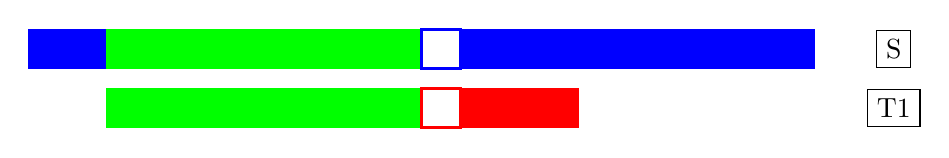
\begin{tikzpicture}

\fill[blue, very thick] (0,0) rectangle (1, 0.5);
\fill[green, very thick] (1,0) rectangle (5, 0.5);
\draw[blue, very thick] (5,0) rectangle (5.5, 0.5);
\fill[blue, very thick] (5.5,0) rectangle (10, 0.5);
\node at (11, 0.25)[draw]  {S};

\fill[green, very thick] (1, -0.75) rectangle (5, -0.25);
\draw[red, very thick](5, -0.75) rectangle (5.5, -0.25);
\fill[red, very thick] (5.5, -0.75) rectangle(7, -0.25);

\node at (11, -0.5)[draw] {T1};
\end{tikzpicture}

\pause

由于红蓝方块位置的字符不匹配,因此需要合理向右移动\textit{T}字符串,在成功匹配了绿色方块位置的字符之后,才可以继续向后匹配:

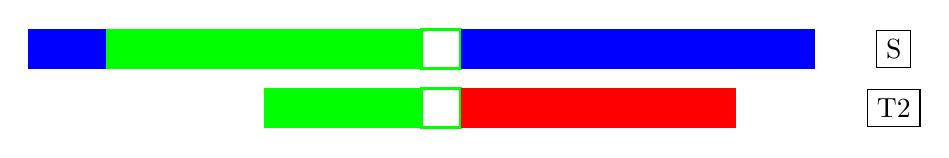
\begin{tikzpicture}

\fill[blue, very thick] (0,0) rectangle (1, 0.5);
\fill[green, very thick] (1,0) rectangle (5, 0.5);
\draw[green, very thick] (5,0) rectangle (5.5, 0.5);
\fill[blue, very thick] (5.5,0) rectangle (10, 0.5);
\node at (11, 0.25)[draw]  {S};

\fill[green, very thick] (3, -0.75) rectangle (5, -0.25);
\draw[green, very thick](5, -0.75) rectangle (5.5, -0.25);
\fill[red, very thick] (5.5, -0.75) rectangle(9, -0.25);

\node at (11, -0.5)[draw] {T2};
\end{tikzpicture}
\pause

此时可以清晰的看到,\textit{T2}绿条部分,恰好是\textit{T1}绿条部分的Border。

也就是说,当遇到匹配失败的字符时,只需要考虑Border所有的长度即可,非Border长度一定不会匹配的更“远”。

\end{block}
    
\end{frame}

\begin{frame}{字符串匹配}

\begin{block}{KMP匹配的复杂度分析}

使用KMP进行字符串匹配时,利用势能分析,不难看出总势能为\textit{|S|},再加上预处理\textit{T}的\textit{next}数组,复杂度为$O(|S| + |T|)$。

\end{block}

\end{frame}

\begin{frame}{例题4}
    
\begin{block}{\href{https://ac.nowcoder.com/acm/problem/14694}{牛客14694}}
给出两个正整数数组$A$和$B$,长度分别为$n\leq m \leq 2\cdot 10^5$,求$A$有多少个长度为$m$的区间$A'$满足:$(A'[1] + B[1])\% k = (A'[2] + B[2])\% k = \dots (A'[m] + B[m])\%k$
\end{block}    

\pause

\begin{block}{题解}

要求满足的条件为:
\begin{enumerate}
    \item [(1)]$(A'[1] + B[1]) \% k = (A'[2] + B[2]) \% k$
    \item [(2)]$(A'[2] + B[2]) \% k = (A'[3] + B[3]) \% k$ \\ $\dots$
    \item [(m)]$(A'[m-1] + B[m-1]) \% k = (A'[m] + B[m]) \% k$
\end{enumerate}

\end{block}

\end{frame}

\begin{frame}{例题4}
    
\begin{block}{题解}

移项得到:
\begin{enumerate}
    \item [(1)]$(A'[1] - A'[2]) \% k = {\color{red}-} (B[1] - B[2]) \% k$
    \item [(2)]$(A'[2] - A'[3]) \% k = {\color{red}-} (B[2] - B[3]) \% k$ \\ $\dots$
    \item [(m)]$(A'[m-1] - A'[m]) \% k = {\color{red}-} (B[m-1] - B[m]) \% k$
\end{enumerate}

\pause

\hphantom{}

因此答案等于${\color{red}-}Diff_B$数组在$Diff_A$数组中的出现次数。

进而问题转化为字符串匹配问题,可以使用KMP解决。

\end{block}

\end{frame}


\begin{frame}{拓展}

\begin{block}{Border的性质}

周期定理:若$p,q$均为串\textit{S}的周期,则$(p,q)$也为\textit{S}的周期。

\hphantom{ }

一个串的Border数量是$O(N)$个,但他们组成了$O(logN)$个等差数列。

\end{block}

\begin{block}{KMP的推广}

拓展KMP(a.k.a Z算法)

\hphantom{}

KMP自动机,Border树

\hphantom{}

AC自动机,即KMP的多串模式。

\hphantom{}

Trie图,即KMP自动机的多串模式。

\end{block}
    
\end{frame}

\end{document}	% Done!